\documentclass{article}
\usepackage{geometry}
\usepackage{amsmath}
\usepackage{graphicx}
\usepackage{caption}
\usepackage{minted}

\renewcommand{\figurename}{Obrázok}

\graphicspath{ {../images/} }

\geometry{margin=0.75in}


\begin{document}

\title{Riešenie 4. úlohy kategórie A}
\author{Jozef Komáromy}

\maketitle

Všetky programy sú zapísané v jazyku Python s predpokladom čísla $n$ uloženého v premennej $N$. V programoch sú použité nedefinované funkcie $Write$ a $Read$ rovnako ako v študijnom text v zadaní.

\section*{Podúloha A}

Všetky prvky vypíšeme po riadkoch jednoduchou iteráciou súradnice $y$ (poradie riadku, začína nulou) od $0$ po $N-1$ a iteráciou súradnice $x$ (poradie stĺpca, začína nulou) od $0$ po $N-1$ pre každú súradnicu $y$. Pre každý prvok vypočítame jeho poradie na disku vzťahom $i = y * N + x$. Nasledovne toto poradie použijeme ako argument pre funkciu $Read$ aby sme získali v poradí $i$-tý blok dát z disku ($blok = Read(i)$). Tento blok vypíšeme funkciou $print$ (\(print(blok)\)). Aby funkcia $print$ neukončila riadok a vypísala medzeru medzi prvkami, použijeme argument \(end = " "\). Celý tento proces spojíme do jedného riadku ako \(print(Read(y * N + x), end = "\ ")\). Po vypísaní každého prvku v jednom riadku (po konci vnútorného for cyklu) ukončíme riadok.

\begin{minted}{python}
for y in range(N):
  for x in range(N):
    print(Read(y * N + x), end = " ")
  print("", end = "\n")
\end{minted}

\section*{Podúloha B}

Riešenie tejto podúlohy bude podobné ako riešenie podúlohy A. Narozdiel od podúlohy A budeme vypisovať stĺpce ako riadky. Aby sme toto dosiahly, stačí len zameniť vonkajší cyklus za vnútorný tak aby sme pre každú súradnicu $x$ vypísali všetky prvky od $y = 0$ až po $y = N-1$. Vzťah pre výpočet poradia zostane rovnaký.

\begin{minted}{python}
for x in range(N):
  for y in range(N):
    print(Read(y * N + x), end = " ")
  print("", end = "\n")
\end{minted}

\section*{Podúloha C}

\subsection*{Jednoduché riešenie}

\textbf{Toto riešenie je použité len ako príklad, nie je mojím konečným riešením pre túto podúlohu.}
\newline
Najjednoduchším riešením by bolo prečítať maticu po stĺpcoch zo dola hore a z ľava do prava a v tom istom poradí ako ju čítame ju zapísať na disk za pôvodnú maticu. Potom by sme túto otočenú maticu znovu prepísali na pôvodné miesto. Tento spôsob je však veľmi neefektívny, pretože je potrebné s každým prvkom matice urobiť 4 operácie na disku, ktoré sú oveľa pomalšie ako operácie s pamäťou. Tento spôsob taktiež potrebuje aby sa na disku bolo dostatočné voľné miesto pre druhú maticu rovnakých rozmerov.

\begin{minted}{python}
for y in range(N):
  for x in range(N):
    Write(N * N + y * N + x, Read(x * N + (N - y - 1)))

for i in range(N * N):
  Write(i, Read(N * N + i))
\end{minted}

\subsection*{Efektívne riešenie}

Aby bolo riešenie efektívne, nechceme aby používalo viac miesta na disku ako zaberá pôvodná matica.
Aby sme otočili maticu bez ukladania údajov na disk, budeme postupne otáčať páry každých štyroch prvkov v smere hodinových ručičiek.

\begin{figure}[h]
  \centering
  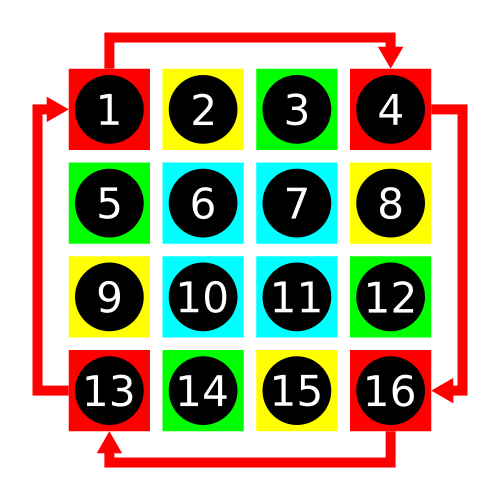
\includegraphics[width=0.35\textwidth]{process}
  \caption{Proces otáčania matice}
\end{figure}

Na obrázku 1 je znázornený proces otáčania matice s rozmerom $n = 4$. Najskôr začneme prvkom v ľavom hornom rohu, presunieme ho do pravého horného rohu, prvok z pravého horného rohu presunieme do pravého dolného rohu, prvok z pravého dolného rohu do ľavého doného rohu, a nakoniec sa vrátime na začiatok do ľavého horného rohu, kde umiestnime prvok z ľavého dolného rohu. Takto sme otočili jednu štvoricu prvkov. Ďalej postúpime k žltej štvorici prvkov. Spravidla začíname tento postup pre štvoricu prvkov od prvku nachádzajuceho sa na hornej strane matice/vnútornej pod-matice. V prípade žltej štvorice teda začneme s prvkom $2$ a postupujeme v poradí $2, 8, 15, 9$. Takto budeme postupovať pre každý prvok hornej strany matice okrem posledného, ktorý už bol otočený s prvým. Keď prejdeme prvý riadok, posunieme sa na ďaľší. Prvý prvok ďaľšieho riadku už bol otočený pri otáčaní prvkov predchádzajúceho riadku. Preto sa vždy na novom riadku presunieme o jeden prvok do prava (ak číslujeme riadky od $1$, na riadku $y$ začneme prvkom $y$-tým v poradí). Posledny prvok na riadku ktorý otočíme je prvok ($n - y - 1$)-tý v poradí. Posledný prvok ktorý otočíme sa nachádza na poslednom riadku hornej polovice matice. Ak je rozmer matice párne číslo, bude to riadok $\frac{n}{2}$, ak je nepárny bude to riadok $\frac{n - 1}{2}$, alebo všeobecne $\left \lfloor \frac{n}{2} \right \rfloor$. Pre ktorýkoľvek prvok vieme vypočítať jeho novú pozíciu ($2$-rozmernú) po otočení vzťahom $x = n - y_0$ a $y = x_0$, kde $x_0$ a $y_0$ sú pôvodnou pozíciou prvku pred otočením.

\subsubsection*{Algoritmus vo forme pythonového programu}

Aby sme mohli otáčať štvorice prvkov, potrebujeme premennú v pamäti do ktorej budeme dočasne ukldať posledný prvok - premmenná $blok$.

\begin{minted}{python}
blok = None
\end{minted}

Hlavný algoritmus bude najskôr iterovať od prvého riadku (index $0$) po riadok $\left\lfloor\frac{n}{2}\right\rfloor$ (index $N // 2 - 1$), tento index uložíme do premennej $sy$. Pre každý riadok bude iterovať cez prvky ktoré treba otočiť: od $y$-tého prvku (index $sy$) po prvok ($n - y - 1$)-tý (index $N - sy - 2$), tento index je premmená $sx$.

\begin{minted}{python}
for sy in range(0, (N // 2 - 1) + 1):
  for sx in range(sy, (N - sy - 2) + 1):
\end{minted}

Premenné $sy$ a $sx$ prepíšeme do premenných $y$ a $x$ aby sme ich mohli modifikovať.

\begin{minted}{python}
    y = sy
    x = sx
\end{minted}

Teraz 5 krát zopakujeme nasledujúci proces: za prvok na pozícií $y, x$ dosadíme prvok uložený v premennej $blok$, do premennej $blok$ zapíšeme pôvodnú hodnotu prvku aby sme ju mohli v ďalšiom kroku cyklu preniesť na ďaľšiu pozíciu. Aby sme mohli takto vymeniť hodnoty v pamäti a disku, použijeme dočasnú premennú $tblok$. 1-rozmerná pozícia na disku z ktorej budeme čítať a zapisovať je vyjadrená vzťahom $y * N + x$.

\begin{minted}{python}
    for i in range(5):
      tblok = Read(y * N + x)
      Write(y * N + x, blok)
      blok = tblok
\end{minted}

Vypočítame ďaľšiu pozíciu s pomocou dočasných premenných $y_0$ a $x_0$.

\begin{minted}{python}
      x0 = x
      y0 = y
      x = N - y0 - 1
      y = x0
\end{minted}

V piatom kroku sa cyklus vráti naspäť na prvú pozíciu a zapíšeme do nej prvok prenesený z poslednej.
Po skončení algoritmu budeme mať na mieste pôvodnej matice v disku otočenú maticu.

\subsubsection*{Časová náročnosť a využitie pamäte}

Algoritmus využíva rovnaké množstvo pamäte nezávisle od rozmeru matice, nepotrebuje viac miesta na disku ako zaberá pôvodná matica. Počet vykonaných zápisov na disk je $5$ pre každú otočenú štvoricu prvkov, takže $5*\frac{n^2}{4}$ pre párne $n$ a $5*\frac{n^2 - 1}{4}$ (pretože stredný prvok otočiť netreba) pre nepárny rozmer $n$, alebo všeobecne $5*\left\lfloor\frac{n^2}{4}\right\rfloor$. Počet prečítaní z disku je rovnaký ako zápisov. Časová komplexita algoritmu je $O(n^2)$. Tento algoritmus je možné upraviť tak aby pre štvoricu zapísal a prečítal z disku len 4 krát.

\subsubsection*{Optimalizovaný program}

\begin{minted}{python}
blok, tblok, x0, y0 = None, None, None, None

for sy in range(0, (N // 2 - 1) + 1):
  for sx in range(sy, (N - sy - 2) + 1):
    blok = Read(sy * N + sx)
    x = N - sy - 1
    y = sx
    for i in range(3):
      tblok = Read(y * N + x)
      Write(y * N + x, blok)
      blok = tblok
      x0 = x
      y0 = y
      x = N - y0 - 1
      y = x
    Write(sy * N + sx, blok)
\end{minted}

\end{document}
